\documentclass{standalone}
\usepackage{graphicx}	
\usepackage{amssymb, amsmath}
\usepackage{color}

\usepackage{tikz}
\usetikzlibrary{intersections, backgrounds}
\usepackage{pgfmath}

\definecolor{light}{RGB}{220, 188, 188}
\definecolor{mid}{RGB}{185, 124, 124}
\definecolor{dark}{RGB}{143, 39, 39}
\definecolor{highlight}{RGB}{180, 31, 180}
\definecolor{gray10}{gray}{0.1}
\definecolor{gray20}{gray}{0.2}
\definecolor{gray30}{gray}{0.3}
\definecolor{gray40}{gray}{0.4}
\definecolor{gray60}{gray}{0.6}
\definecolor{gray70}{gray}{0.7}
\definecolor{gray80}{gray}{0.8}
\definecolor{gray90}{gray}{0.9}
\definecolor{gray95}{gray}{0.95}

\newcommand*{\offset}{0.025}

\begin{document}

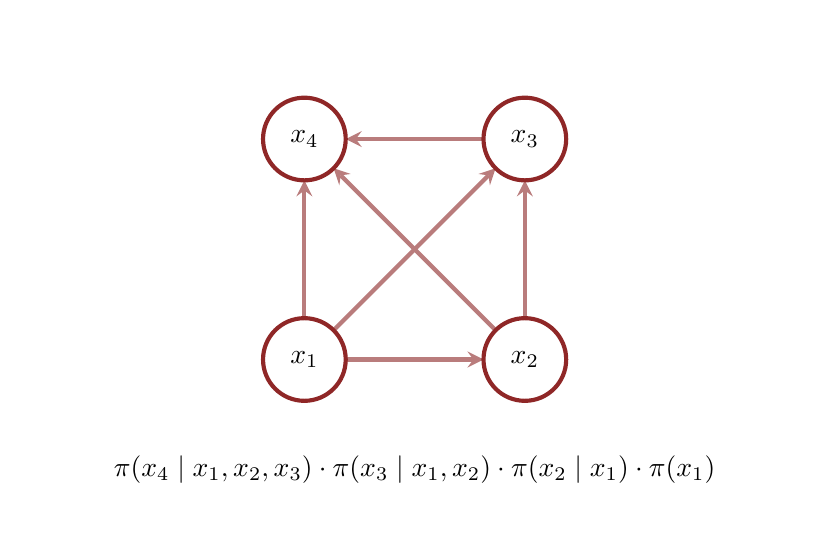
\begin{tikzpicture}[scale=0.35, thick]

\pgfmathsetmacro{\r}{1.5}

% One
\pgfmathsetmacro{\dx}{0}
\pgfmathsetmacro{\dy}{0}

\draw[white] (-14 + \dx, -10 + \dy) rectangle (14 + \dx, 8 + \dy);

\draw[->, >=stealth, color=mid, line width=1.5] (-4 + \dx, -4 + \dy) -- (4 - \r + \dx, -4 + \dy);
\draw[->, >=stealth, color=mid, line width=1.5] (-4 + \dx, -4 + \dy) -- (-4 + \dx, 4 - \r + \dy);
\draw[->, >=stealth, color=mid, line width=1.5] (-4 + \dx, -4 + \dy) -- ({4 - \r * cos(45) + \dx}, {4 - \r * sin(45) + \dy});

\filldraw[fill=white, draw=dark, line width=1.5] (-4 + \dx, -4 + \dy) circle (\r)
node[color=black] { $x_{1}$ };

\draw[->, >=stealth, color=mid, line width=1.5] (4 + \dx, -4 + \dy) -- (4 + \dx, 4 - \r + \dy);
\draw[->, >=stealth, color=mid, line width=1.5] (4 + \dx, -4 + \dy) -- ({-4 + \r * cos(45) + \dx}, {4 - \r * sin(45) + \dy});

\filldraw[fill=white, draw=dark, line width=1.5] (4 + \dx, -4 + \dy) circle (\r)
node[color=black] { $x_{2}$ };

\draw[->, >=stealth, color=mid, line width=1.5] (4 + \dx, 4 + \dy) -- (-4 + \r + \dx, 4 + \dy);

\filldraw[fill=white, draw=dark, line width=1.5] (4 + \dx, 4 + \dy) circle (\r)
node[color=black] { $x_{3}$ };

\filldraw[fill=white, draw=dark, line width=1.5] (-4 + \dx, 4 + \dy) circle (\r)
node[color=black] { $x_{4}$ };

\node[] at (0 + \dx, -8 + \dy) {$\pi(x_{4} \mid x_{1}, x_{2}, x_{3}) \cdot \pi(x_{3} \mid x_{1}, x_{2}) \cdot \pi(x_{2} \mid x_{1}) \cdot \pi(x_{1})$};

\end{tikzpicture}

\end{document}  